\fig{fv:h1:expansion}{自由杆的原长与伸长分开标记；图中伸长夸张绘制}{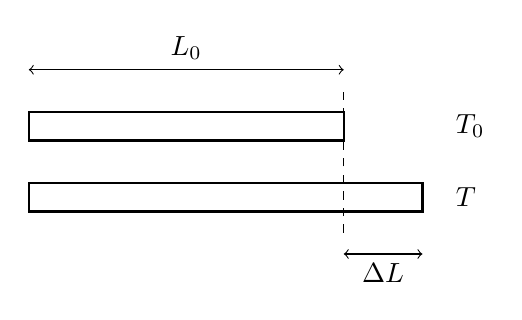
\begin{tikzpicture}[x=1cm,y=.9cm]
\draw[thick](0,1)rectangle(4,1.4);\draw[thick](0,0)rectangle(5,.4);\draw[dashed](4,-.3)--(4,1.7);
\draw[<->](0,2)--(4,2)node[midway,above]{$L_0$};\draw[<->](4,-.6)--(5,-.6)node[midway,below]{$\Delta L$};
\node[right]at(5.3,1.2){$T_0$};\node[right]at(5.3,.2){$T$};\end{tikzpicture}}
图\ref{fv:h1:expansion}中两次长度共用同一左端基准，虚线保留原右端的位置，向右多出的一段才是$\Delta L$。相对伸长应除以原长$L_0$；不能将升温后的$L$误作基准长度。若两端都受固定限制，图示自由伸长便不能实际发生，应另列约束和弹性关系。
